%%% Add [final] option to the report class to switch between draft and final version of the report
%%% Use [narrowmargin] to enable narrow margins - this may impair readability.
\documentclass[a4paper, 12pt]{include/compassreport}   %Or compasslargereport if chapters are required.
  
\reportnumber{DXX}
\reporttitle{Simulator/Animator Design Document}
\shortreporttitle{Simulator/Animator Design}  %To use if report title is too long for header

%%% Set document release class as appropriate
%%% e.g. Public, Restricted, Programme Participant
\reportstatus{Public}


%%% If document is a deliverable, this flag should be commented out 
%%% e.g. %\technotetrue
%%% If report is a technical report, leave uncommented
%%% e.g. \technotetrue
\technotetrue % Comment out as appropriate

\submissiondate{Month Year}
\contributors{
  Anders Kaels Malmos, AU 
}
\editors{
  Peter Gorm Larsen, AU
}
\reviewers{}


%% Version details  
% #1: version
% #2: date
% #3: author
% #4: description
\addversion{0.1}{25-04-2013}{Anders Kaels Malmos}{Initial document version}
%\addversion{0.2}{dd-mm-yyyy}{Richard Payne}{Second version}
  
\begin{document}
\maketitle


%%%% Document abstract page %%%% 
\section*{Abstract}
\label{sec:abstract}

This document describes the overall design of the CML
simulator/animator and provides an overview of the code structure
targeting developers.

\newpage

%%%% Document table of contents page %%%% 
\tableofcontents
\newpage

%%%% Document Content %%%% 
%% \chapter{Chapter Title} %% if compasslargereport is in use
\section{Preface}
This document is targeted at developers and describes the overall
strucure and design of the CML simulator, it is not a detailed
description of each component. This kind of documentation is done in
Javadoc and can be generated automatically from the code.

% \section{Introduction}
% \label{sec:introduction}

% The implementation described here is an implementation CML simulator is one

\section{Overall Structure}
\label{sec:introduction}
This section describes the overall source code structure of the CML
interpreter. At the top level the code can be split up in two separate
components:

\begin{description}
\item[Core component] Implements the operational semantics that are
defined in \cite{D23.3} and is located in the java package named
\emph{eu.compassresearch.core.interpreter}
\item[IDE component] Exposes the core component to the Eclipse
framework as an integrated debugger. It is located in the
\emph{eu.compassresearch.ide.cml.interpreter\_plugin} package.
\end{description}

Each of these components will be described in further detail in the
following sections.

\subsection{The Core Structure}

The design philosophy of the top-level structure is to encapsulate all
the classes and interfaces that makes up the implementation of the
core functionality and only expose those that are needed to utilize
the interpreter. This provides a clean separation between the
implementation and interface and makes it clear for both the users,
which not necessarily wants to know about the implementation details,
and developers which parts they need to work with.
 
The following packages defines the top level structure of the core:
\begin{description}
\item[eu.compassresearch.core.interpreter.api] This package and
  sub-packages contains all the public classes and interfaces that
  defines the API of the interpreter. This package includes the main
  interpreter interface \textbf{CmlInterpreter} along with additional
  interfaces.
  The api sub-packages groups the rest of the API classes and
  interfaces according to the responsibility they have.

\item[eu.compassresearch.core.interpreter.api.behaviour] This package
  contains all the components that define any CML behavior. A CML
  behaviour is either an observable event like a channel synchronization
  or a internal event like a change of state. The main interface is
  \textbf{CmlBehaviour}.

\item[eu.compassresearch.core.interpreter.api.events] This package
  contains all the public components that enable users of the
  interpreter to listen on event from both \textbf{CmlIntepreter} and
  \textbf{CmlBehaviour} instances.

\item[eu.compassresearch.core.interpreter.api.transitions] This
  package contains all the possible types of transitions that a
  \textbf{CmlBehaviour} instance can make. This will be explained in
  more detail in section \ref{sec:transition_structure}.

\item[eu.compassresearch.core.interpreter.api.values] This package
  contains all the values used in the CML interpreter. Values are used
  to represent the the result of an expression or the current state of a
  variable.

\item[eu.compassresearch.core.interpreter.debug] TBD

\item[eu.compassresearch.core.interpreter.utility] The utility
packages contains components that generally reusable classes and
interfaces. 

\item[eu.compassresearch.core.interpreter.utility.events] This package
contains components helps to implement the Observer pattern. 

\item[eu.compassresearch.core.interpreter.utility.messaging] This
  package contains components to pass message along a stream.



\item[eu.compassresearch.core.interpreter] This package contains all
  the classes and interfaces that defines the core functionality of the
  interpreter. The important class for any user of the interpreter is
  the \textbf{VanillaInterpreteFactory} that creates
  \textbf{CmlInterpreter} instances.

\end{description}

The reason for this top level structure is to encapsulate all the
classes and interfaces that makes up the core functionality of the
interpreter and only expose the classes and interfaces that are needed
to utilize it without knowing the details. This provides a clean
separation between the implementation and the public interface.

The eu.compassresearch.core.interpreter package are split into several
folders, each representing a different logical component. The
following folders are present

\begin{description}
\item[cml] 
\item[visitors]
\item[util]
\item[debug]
\item[...]
\end{description}

\subsection{The IDE Structure}

%\subsection{Subsection}
%\label{sec:subsection-1.1}

\section{Simulation/Animation}
This section describes the static and dynamic structure of the
components involved in simulating/animating a CML model.

\subsection{Static Structure}
\label{sec:dynamic_structure}
The top level interface of the interpreter is depicted in figure
\ref{fig:interpreter_topLevelStructure}, followed by a short
description of each the depicted components.
\begin{figure}[ht!]
  \begin{center}
    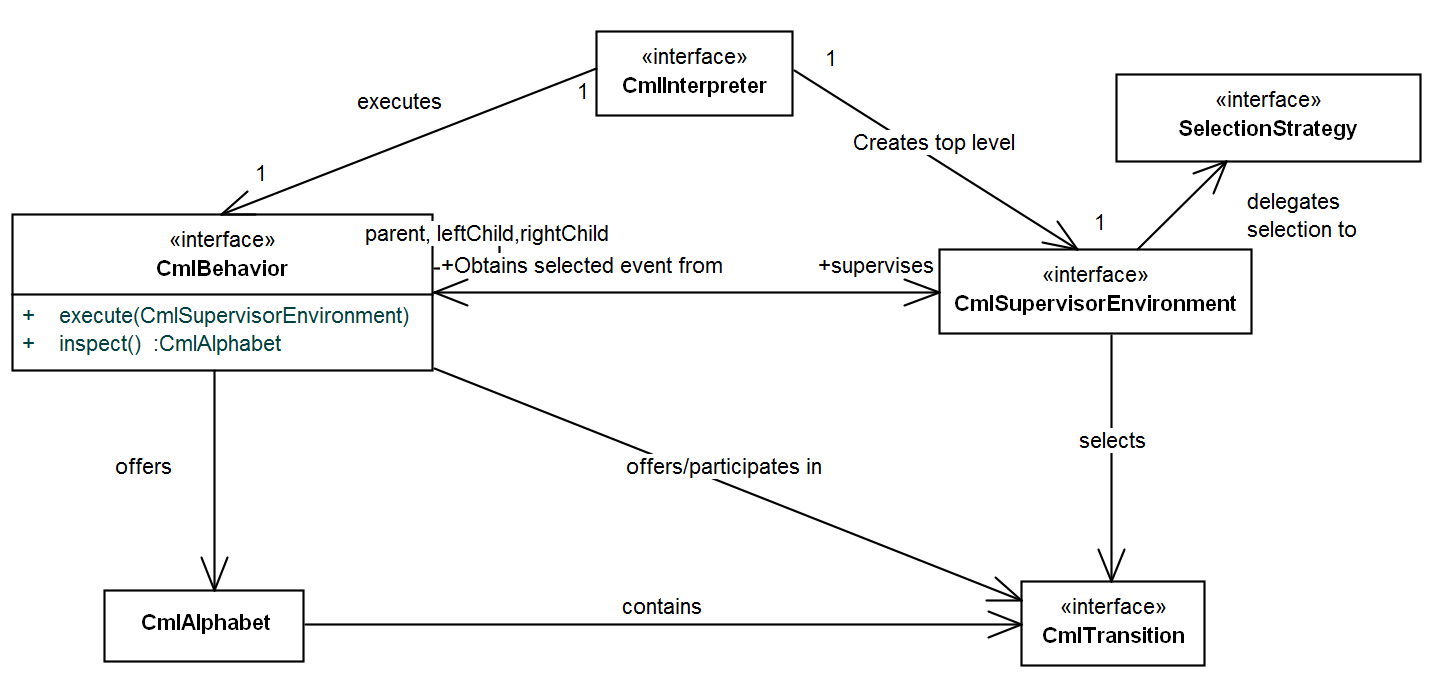
\includegraphics[width=1\textwidth]{figures/toplevelStructure}
    \caption{The high level classes and interfaces of the interpreter core component}
    \label{fig:interpreter_topLevelStructure}
  \end{center}
\end{figure}

\begin{description}
\item[CmlInterpreter] The main interface exposed by
  the interpreter component. This interface has the overall
  responsibility of interpreting. It exposes methods to execute, listen
  on interpreter events and get the current state of the interpreter. It
  is implemented by the \textbf{VanillaCmlInterpreter} class.
\item[CmlBehaviour] Interface that represents a behaviour specified by
  either a CML process or action. It exposes two methods: \emph{inspect}
  which calculates the immediate set of possible transitions that the
  current behaviour allows and \emph{execute} which takes one of the
  possible transitions determined by the supervisor. A specific
  behaviour can for instance be the prefix action ``a -> P'', where the
  only possible transition is to interact in the a event.  in any
\item [CmlSupervisorEnvironment] Interface with the responsibility of
  acting as the supervisor environment for CML processes and actions. A
  supervisor environment selects and exposes the next transition/event
  that should occur to its pupils (All the CmlBehaviors under its
  supervision). It also resolves possible backtracking issues which
  may occur in the internal choice operator. 
\item[CmlEventSelectionStrategy] This interface has the responsibility
  of choosing an event from a given CmlAlphabet. This responsibility is
  delegated by the CmlSupervisorEnvironment interface.
\item[CmlTransition] Interface that represents any kind of transition that
  a CmlBehavior can make. This structure will be described in more
  detail in section \ref{sec:event_structure}.
\item[CmlAlphabet] This class is a set of CmlTransitions. It exposes
  convenient methods for manipulating the set.
\end{description}

To gain a better understanding of figure
\ref{fig:interpreter_topLevelStructure} a few things needs
mentioning. First of all any CML model (at least for now) has a top
level Process. Because of this, the interpreter need only to interact
with the top level CmlBehaviour instance. This explains the one-to-one
correspondence between the CmlInterpreter and the
CMLBehaviour. However, the behavior of top level CmlBehaviour is
determined by the binary tree of CmlBehaviour instances that itself
and it's child behaviours defines. So in effect, the CmlInterpreter
controls every transition that any CmlBehaviour makes through the top
level behaviour.

\subsubsection{Transition Structure}
\label{sec:transition_structure}

As described in the previous section a CML model is represented by a
binary tree of CmlBehaviour instances and each of these has a set of
possible transitions that they can make. A class diagram of all the
classes and interfaces that makes up transitions are shown in figure
\ref{fig:events}, followed by a description of each of the elements.

A transition can be either observable or silent. An observable
transition occurs either when time passes or a
communication/synchronization takes place on a channel. All of these
transitions are captured in the ObservableEvent interface. 
A silent transitions is captured by the SilentTransition interface and
can either mark the occurrence of a hidden event or an internal
transition.

\begin{figure}[ht!]
  \begin{center}
    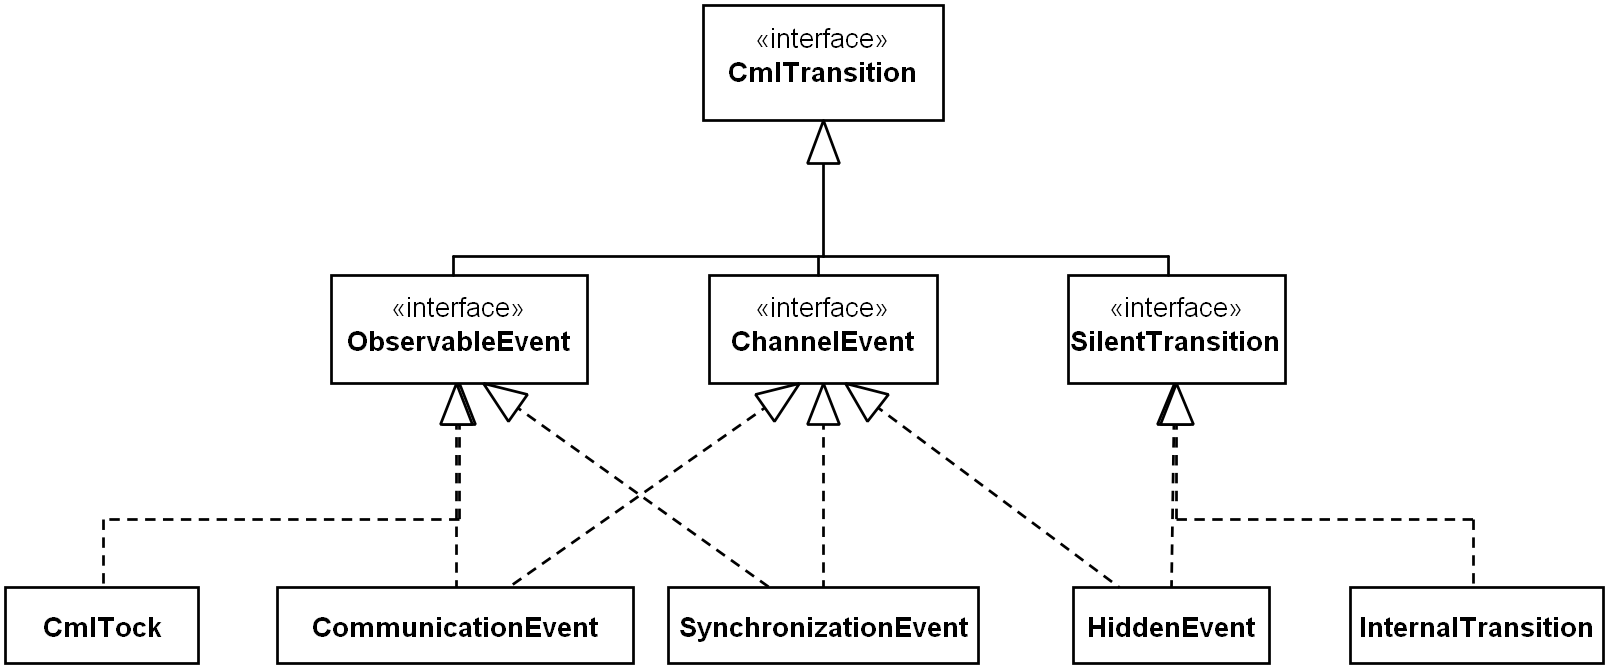
\includegraphics[width=1\textwidth]{figures/Events}
    \caption{The classes and interfaces that defines transitions/events}
    \label{fig:events}
  \end{center}
\end{figure}

\begin{description}
\item[CmlTransition] Represents any possible transition.
\item[ObservableEvent] This represents any observable transition.
\item[ChannelEvent] This represents any event that occurs on a channel.
\item[CmlTock] This represents a Tock event marking the passage of a time unit.
\item[CommunicationEvent] This represents a communication event on a
  specific channel and carries a value to be communicated.
\item[SynchronizationEvent] This represents a synchronization event on
  a specific channel and carries no value.
\item[SilentTransition] This represents any non-observable transition.
\item[HiddenEvent] This represents an observable event that has been hidden by the hiding operator.
\item[InternalTransition] This represents any transition that are
  internal to a process, like assignemnt, the invocation of a method and
  etc.
\end{description}

\subsubsection{Action/Process Structure}
\label{sec:action_process_structure}
Actions and processes are both represented by the CmlBehaviour
interface. A class diagram of the important classes that implements
this interface is shown in figure \ref{fig:cmlbehaviors}
\begin{figure}[ht!]
  \begin{center}
    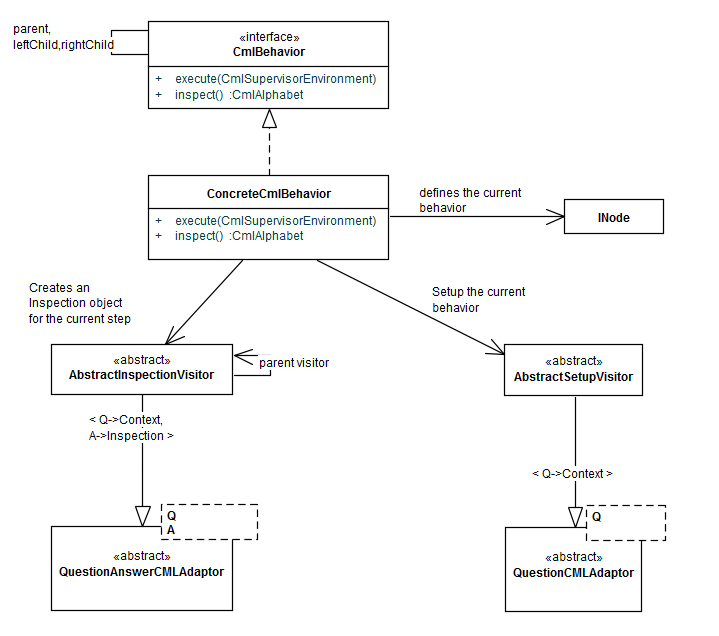
\includegraphics[width=0.9\textwidth]{figures/CmlBehaviors}
    \caption{The implementing classes of the CmlBehavior interface}
    \label{fig:cmlbehaviors}
  \end{center}
\end{figure}

As shown the \textbf{ConcreteCmlBehavior} is the implementing class of
the CmlBehavior interface. However, it delegates a large part of its
responsibility to other classes. The actual behavior of a
ConcreteCmlBehavior instance is decided by its current instance of the
INode interface, so when a ConcreteCmlBehavior instance is created a
INode instance must be given. The INode interface is implemented by
all the CML AST nodes and can therefore be any CML process or action.
The actual implementation of the behavior of any process/action is
delegated to three different visitors all extending a generated
abstract visitor that have the infrastructure to visit any CML AST
node.

The following three visitors are used:  
\begin{description}
\item[AbstractSetupVisitor] This has the responsibility of performing
  any required setup for every behavior. This visitor is invoked
  whenever a new INode instance is loaded.
\item[AbstractEvaluationVisitor] This has the responsibility of
  performing the actual behavior and is invoked inside the execute
  method. This involves taking one of the possible transitions.
\item[AbstractAlphabetVisitor] This has the responsibility of
  calculating the alphabet of the current behavior and is invoked in the
  inspect method.
\end{description}



\begin{figure}[ht!]
  \begin{center}
    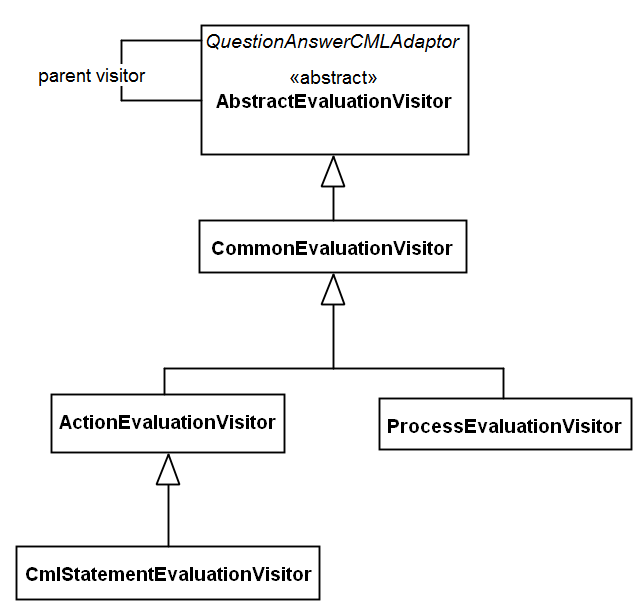
\includegraphics[width=1\textwidth]{figures/Visitors}
    \caption{Visitor structure}
    \label{fig:visitors}
  \end{center}
\end{figure}



\subsection{Dynamic Structure}
\label{sec:dynamic_structure}


%%%% Bibliography %%%%
\newpage
\bibliographystyle{alpha}
\bibliography{bibliography} 
\label{ch:bib} %label to refer to


\end{document}  